\documentclass[titlepage,a4paper,12pt]{book}

\usepackage[utf8]{inputenc}
\usepackage[catalan]{babel}
\usepackage{graphicx}
\usepackage{marvosym}
\usepackage{listings}
\usepackage{textcomp}
\usepackage[]{color}
\begin{document}
\tableofcontents
\section{Introducció} % (fold) Objectius?
	\label{sec:Introduccio}
	Un altre problema on hem aplicat Algoritmes evolutius és en el descobriment
	de fàrmacs \texttt{de novo}.  \texttt{De novo} és el nom que es dóna a les
	tècniques relacionades amb el descobriment de 0, és a dir, on no es té
	prèviament cap lligand a imitar.

	La situació és la següent.  En determinades situacions, es disposa d'un
	esquelet o \textit{scaffold} que se sap que té certa activitat, però no es
	disposa amb seguretat de alguns \textit{radicals} , que són les parts de la
	molècula que, sense canviar la seva estructura general, ni la seva
	activitat, faran que es pugui 'enganxar' millor en el lligand.  Els radicals
	que poden anar en cada posició són coneguts (en la majoria de casos).

	En certa manera, podriem dir que és com ``decorar'' un esquelet de la
	molècula per a fer-lo més apte per a enganxar-se amb el seu target o diana.

	Un dels problemes que tenen els mètodes actuals són els grans costos
	que es deriven d'aquest procés, ja que el que es fa és sintetitzar TOTES les
possibles variants i combinacions de radicals, i mesurant la energia %XXX (disipada?)
	s'intenta buscar la que minimitza aquesta.

	si tenim un esquelet com el següent, amb 3 Radicals, i 4 posibles ``building
	blocs'' per a cada R, la (ombinatioria ens dóna que necessitarem sintetitzar
	aproximadament $4^3 = 64 $, però si el número creix una mica, el creixement
	és exponencial, fent molt costós el procediment seguint aquest mecanisme.

	Si pensem que la qualitat del resultat evaluat és en funció dels Radicals
	escollits per a cada R1..RN, podem anar una mica més enllà i intentar fer
	una aplicació que ens aujudi i ens guii a trobar un lligand amb bona
	activitat explorant només una petita part de l'espai de cerca.
	
	\texttt{La idea en aquest programa és doncs, construir un algoritme genètic
	semi-interactiu que ens permeti arribar a la millor tria de radicals (o
		alguna de molt bona) sintetitzant una petita part del espai de búsqueda.}

	Per a evaluar la qualitat de una combinació, no hi ha més remei que
	sintetitzar la molècula en qüestió en el laboratori i retornar el resultat.
	Així doncs, es tracta d'un algorisme genètic interactiu %XXX ref a paper.
	que ens guiarà les proves que hem de fer a través dels creuaments i les
	mutacions, trobant ``relacions'' (epistàcia) entre els diferents radicals, i
	aconseguint resultats bons explorant una petita part del espai de búsqueda.

	Una altra objectiu d'aquest programa, ha estat convertir-lo en un
	``framework'' d'algorismes genètics.  Veient que la funció de fitness és una
	funció que executa l'usuari, i ell és qui puntúa cadascuna de les
	combinacions, s'ha intentat anar més enllà i aconseguir una aplicació que
	pugui ser utilitzada no només en aquest context, sinó en cualsevol que ens
	podem trobar en un futur, sempre i quan requereixi uns operadors similars.

	Una altra manera d'imaginarse aquest enfoc \texttt{meta} és pensar-ho com si
	separéssim la funció fitness de la resta del procés d'algoritme genètic.
	L'únic que necesita el algoritme genètic és un receptor de dades, que
	donada una entrada, hi doni una sortida.  Si es mira d'aquesta manera, no
	estem fent més que desacoblar la evaluació del procés de creuaments,
	mutacions i reproducció.

	Fins a aquest punt, podríem utilitzar algun sistema amb callbacks, on
	l'usuari simplement entri els fitness als diferents individuus (combinacions
	de radicals), però com que la evaluació no és instantanea, el programa no
	pot ser interactiu en el sentit clàssic del terme (inici-interacció-fi),
	sinó que ha de permetre aturar-se i més endevant, tornar a rependre el curs
	del algoritme evolutiu. 

	Una vegada estem en aquest punt, la següent evolució lògica és la
	deslocalització també espaial de les 2 parts.  Donat que el procés
	d'evaluació d'una combinació de erres donada pot trigar dies, el coll
	d'ampolla serà clarament aquest, permetent-nos així separar algorisme
	genètic i Fitness a través d'una xarxa, i permetent convertir el sistema en
	un servei web, accessible des d'arreu del món.

	Tot i que la gestió d'això només ens implica implementar el sistema com a
	servei web (SOAP) i tenir una bona gestió d'usuaris i projectes, es veu
	clarament que el que comença essent una aplicació per a solucionar un
	problema concret, s'ha anat abstraient i generalitzat fins al punt de
	convertir-se en un programa molt més potent, ja que ara abarca un espectre
	molt més gran de problemes pels quals està capacitat resoldre.

	Tot seguit s'expliquen els detalls d'implementació.

% section Introducció (end)

\section{Context Químic} % (fold)
	\label{sec:Context Quimic}

	En el proccés de descobriment de fàrmacs (drug discovery), no només és
	necessari trobar un compost que reaccioni favorablement en una molècula
	objectiu, sinó que també ha de reunir certes condicions per tal que un
	principi actiu es pugui convertir en un fàrmac aplicable.  Aquestes
	condicions son tals com:

	\begin{itemize}
	\item No toxicitat
	\item Que es el cos no el rebutgi
	\item Facilitat d'absorció i estabilitat del nou compost (lligand +
			receptor)
	\end{itemize}

% section Context Químic (end)


\section{Procediment informàtic} % (fold)
\label{sec:Procediment informatic}

En aquesta aplicació, no ha estat tant complex d'implementar l'algorisme genètic
com tot l'entorn (framework) que permet fer del \texttt{core} una part molt
flexible i accessible des de tot arreu (web, consola).

El diseny de \texttt{Chiron}, ha hagut de estar molt pensat, i de fet, s'ha vist
modificat a mesura que avançava la seva implementació per problemes que s'han
trobat en tecnologies que pensàvem que serien suficienment flexibles per a les
nostres necessitats, i després s'ha vist que no eren del tot adecuades per a les
nostres necessitats.

Començarem amb el workflow que ha de permetre Chiron perquè l'usuari pugui
utilitzar-lo fàcilment i n'extraurem els diferents casos d'ús.

Un usuari, en començar un projecte, ha de poder crear un experiment nou.  Aquest
experiment ha d'estar lligat, òbviament a aquest usuari, amb el que ens obliga
també a poder fer altes, baixes i modificacions dels usuaris que tenen accés a
la aplicació.

Les altes, baixes i modificacions de usuaris no les gestiona el propi
\texttt{Chiron}, ja que la aplicació que dona accés a Chiron és qui s'encarrega
de controlar els accessos a aquests.  Chiron únicament utilitza la base dades
aquesta, per saber quin usuari és el que està utilitzant el programa, i fa totes
les accions en el seu nom.

La creació de experiments nous sí que és una labor de Chiron, i és a partir
d'aquest moment on Chiron s'encarrega de registrar els events.

Per a la creació d'un nou experiment, Chiron necessita únicament el número de
Radicals que conté l'esquelet (R1 \dots RN), el número de al·lels diferents que
poden estar en cadascun dels Radicals, el tamany de la població, i un booleà
indicant si volem que chiron recordi (cachegi) els resultats o no.  Amb aquestes
dades, Chiron en té prou per començar l'experiment.  És clar que també demanarà
un nom per al que l'usuari s'hi pugui referir.

En aquest punt, hi ha dues coses que poden sorprendre, i seguidament s'expliquen
els perquès:

\begin{itemize}
	\item \textbf{No necessitem l'scaffold}. Per a Chiron, l'esquelet (scaffold)
	que usem no té la més mínima importància, ja que sempre serà una part fixa,
	i no ens aportarà res per a la nostra aproximació al problema.  És per això
	que el programa, tot i guardar-se'l per a futura referència, no l'usa en tot
	el procés per a fer càlculs.

	\item \textbf{Perquè decidir si guardem els resultats previs?}.
	Aparentment, sempre que calculem un individuu nou, haurñiem de guardar-nos
	els resultats obtinguts per si més endevant surt el mateix element.  El fet
	que ens fa donar-li la opció al usuari és que l'evaluació de la activitat
	d'una molècula, es fa en un laboratori, i segons el tipus d'experiments que
	es fan, els resultats només tenen valor uns en relació amb els altres.  Si
	és així, al usuari no li interessa que es guardin els valors ja calculats,
	ja que si en properes generacions del algorisme genètic torna a apareixer la
	mateixa combinació de erres, s'haurà de calcular de nou.
\end{itemize}

Una vegada l'usuari ha creat el nou experiment, se li proposa unes quantes
molècules a evaluar (tantes com hagi decidit l'usuari com a tamany de la
població).

Al cap d'un temps, quan l'usuari ha evaluat les molècules proposades per Chiron,
aquest retornarà a la interfície de Chiron, identificarà l'experiment, i posarà
valors a cadascuna de les molècules evaluades.  Una vegada les tingui TOTES
evaluades (sinó estan totes, Chiron no deixarà passar d'aquest punt), s'activarà
la opció de \texttt{fer una altra iteració}.  

En aquest punt, a partir de les dades que tenim, Chiron fa una iteració i
presentarà al usuari una nova generació de molècules, fent creuaments i
mutacions sobre les molècules que tinguem evaluades.

Com que el workflow d'aquest programa no és ``continuu'' en el sentit que el
programa es manté viu durant tot el procés, les dades que volem guardar (encara
que siguin només temporals o internes per a un experiment determinat), s'han
d'emmagatzemar en una base de dades, ja que les tècniques de memoizing %apartat pholus
perden la informació d'execució en execució, i no funcionarien en aquest cas.

Per a aquesta tasca s'ha utilitzat un servidor remot MySql.
%estructura de taules

En el cas que en la primera generació no hi hagi cap molècula que presenti la
més mínima activitat (no superen un llindar donat), Chiron no segueix el curs
normal de mutacions i creuaments, ja que això ens dóna lloc a un intent de
convergència que no ens interessa.  Per exemple, si tenim una població de 30
individuus i tots tenen fitness ~0, Chiron intentarà fer creuaments entre ells
aleatoris (ja que cap d'ells guanya sobre els altres).  No només això sinó que
al fer això, molts dels individuus de la següent generació seran iguals als ja
evaluats, ja que hem reduit molt l'espai de búsqueda sobre el que ataquem.

Si evaluéssim funcions matemàtiques contínues i amb un gradient clar fins al
millor resultat (o els millors resultats), no tindríem aquest problema, però els
nostres casos són, en la gran majoría, casos molt difícils, on tenim un espai de
búsqueda molt gran però els pous amb activitat són molt pocs, i hem d'intentar
arribar a aquests pous primer, i després optimitzar per les vies del algoritme
genètic.
%figura de la funcio amb pics

La solució que s'ha adoptat ha estat la de generar una població d'individuus
nova, sense tenir en compte ĺa generació anterior, com si es comencés un
experiment nou.  Fent això evitem que l'Algoritme genètic estigui ``viciat'' de
bon principi, i maximitzem les probabilitats de trobar algun pou d'energia.
% funcions graduals / punxegudes

Les proves de correctesa del programa, s'han fet amb funcions matemàtiques
contínues, per tal de saber del cert que l'algorisme funciona bé.  Els resultats
obtinguts d'aquestes funcions també seràn exposats més endevant en l'apartat de
resultats. 

Hi ha un conjunt de funcions matemàtiques que es consideren ``típiques'' per a
usarles com a toy problems, per exemple, s'ha provat l'algoritme evolutiu
representant una funció on cada al·lel només té dos possibles valors , 0 i 1, i
la funció únicament suma els bits dels cromosomes.  El que es busca en aquesta
funció, és maximitzar o bé minimitzar el resultat de la suma de bits.  Aquest,
tot i ser un exemple gairebé trivial, ens serveix per saber si l'algorisme
evolutiu funciona correctament.  Aquest exemple també ens serveix perquè les
mutacions i creuaments utilitzats són els mateixos que utilitzem en la versió
final de la aplicació.

Els resultats obtinguts són bons, arribant al millor resultat (tot uns) o a un
dels millors explorant només un percentatge de aproximadament el  10\% de
l'espai de búsqueda.

La funció de la suma de bits és una funció trivial per a cualsevol algorisme
evolutiu, donada la seva simplicitat.  És per això que després de provar amb
aquesta funció, hem provat funcions més complicades de trobar, fins a arribar a
les conegudes com a ``funcions trampa''.  Les funcions trampa són funcions que
creem nosaltres, que tenen canvis de pendent, tenint el millor resultat no pas
en un extrem (tot uns o tot zeros), sinó que hi ha una posició del vector que
val més que les altres, o alguna que penalitza.

Una de les funcions trampa que hem provat, és la de mapejar en un vector de bits
una valoració determinada per a cada suma de bits.  Per exemple, donat un vector
de 5 posicions:


 % theme=Berlin;caption_top=1;caption=Exemple tanimotos
 % bits a 1 & valor
 % 0 & 1
 % 1 & 2
 % 2 & 3
 % 3 & 4
 % 4 & 5
 % 5 & 0

\begin{table}
\centering
\caption{Exemple tanimotos}
\begin{tabular}{|r|r|}
\hline
\multicolumn{1}{|c|}{\textbf{bits a 1 }} & \multicolumn{1}{c|}{\textbf{ valor}} \\
\hline
\hline
0 & 1 \\
1 & 2 \\
2 & 3 \\
3 & 4 \\
4 & 5 \\
5 & 0 \\
\hline
\end{tabular}
\end{table}


L'ideal en aquest cas és trobar un vector que té 4 bits a 1 i un a 0.  Això,
clarament és una trampa per a l'algorisme genètic, ja que al fer els creuaments
entre dos cromosomes que tenen una bona puntuació, fa que els resultants, siguin
molt dolents. És una manera d'enganyar al algoritme evolutiu que ens serveix per
a saber si aquest és prou robust per a trobar un resultat bo.  En aquests casos,
l'elitisme, és molt determinant per a obtenir bons resultats.
% section section name (end)

%SOAP PUNT
Un altre aspecte important de Chiron és la versatilitat que té per a executar-se
amb diferents funcions de fitness.  Com s'ha explicat en la introducció del
capítol, Chiron permet evaluar manualment cadascun dels elements.  Donat que una
evaluació d'una molècula pot portar hores o dies, l'algorisme genètic ha de ser
capaç de mantenir l'estat i congelarse a cada iteració.

Les llibreries usades (eodev), estan preparades per a mantenir l'estat en arxius
de text pla, però ho fan en el moment que s'ha acabat de executar la funció
evaluació de tots els individuus d'una generació.  Per a poder aturar la
execució abans (a nivell lògic), el que hem disenyat és un sistema per a
recollir i posar dades automàticament en els arxius de estat.  eodev està
programat en c++, i per tant, la funció de fitness ha de ser sempre la mateixa
ja que només volem tenir una instància de pholus per executar, i no pas una per
a cada projecte que es faci.  El que hem fet per a solucionar aquesta qüestió és
``anul·lar'' la funció de fitness fent que sigui una stub, que dona fitness zero
a tots els individuus que evalua.  Configurant Chiron per a què faci una sola
generació, aconseguim guardar l'estat en un arxiu, amb els paràmetres del
algorisme genètic, les llavors (seed), i els individuus de la generació actual.
Llavors, el programa que executa el core de Chiron pot parsejar l'arxiu, i
insertar els elements en una base de dades (ens interessa tenir un històric de
tots els elements evaluats en generacions prèvies).  Aquests resultats són els
que es presenten al usuari, que pot recuperar cuan vulgui ja que la recuperació
de les dades es fa desde la base de dades MySql.

Quan l'usuari disposa de dades sobre les molècules, les pot introduir a través
d'una interfície, i tornar a executar una generació.

Si l'usuari ha configurat el projecte perquè mantingui els valors d'evaluacions
passades, en el moment que Chiron detecta una molècula que ja ha estat evaluada,
no li presenta al usuari, i és Chiron qui s'encarrgarà de afegir el resultat en
el moment de la següent generació.

%subsub?  PRoblemes d'inicialització.

En  molts casos reals, ens trobem que tenim una immensa majoria de valors iguals
com a resultat de les evaluacions.  Aquests resultats són per les molècules que
o bé no poden ser sintetitzades, o bé no superen un llindar mínim d'activitat.

Això ens ha suposat un gran problema perquè si evaluem la primera generació i
tots els elements tenen el mateix fitness (0), la següent població que Chiron
suggerirà serà una població tal que haurà sortit de creuar i mutar la primera
població aleatoriament entre ella.  Aquest procediment ens provoca una
convergència prematura que no desitgem, ja que el que passa en realitat és que
encara no hem mostrejat cap molècula que ens doni un mínim d'activitat amb el
que poder ``jugar''.

Problemes d'aquestes característiques només es donen en casos on l'espai de
búsqueda és molt gran comparat amb el número de elements que tenen resultats
diferents de 0.

Per exemple, si volguéssim trobar, en el problema de la suma de bits una
configuració concreta (10101), o bé trobar elements amb unes certes
característiques (que sumin 3), i tots els elements que ho compleixen tenen
fitness 1 i els que no, tenen fitness 0, ens trobariem amb problemes similars.

Aquest problema, l'hem solucionat provocant que Chiron resetegi l'experiment
(recordant les molècules evaluades en la base de dades), i torni a donar una
població d'individuus aleatòria.  Així maximitzem les probabilitats de trobar un
o més pous energètics, que son les àrees del espai de búsqueda (normalment
contígues) on es troben els elements amb fitness superiors al llindar.  En el
moment que trobem molècules amb activitat, l'algorisme segueix el procediment
normal.

%BBDD
Per a guardar l'estat del procés, hem creat una base de dades que ens permet
accedir i modificar la informació de un projecte.  La implementació d'aquesta
base de dades la hem fet amb MySql (més endevant es discutirà el perquè de la
elecció d'aquesta tecnologia en front a altres bases de dades, o altres
tècniques per a emmagatzemar dades (com poden ser Tokyo Cabinet/Tyrant, MongoDB
o altres SGBDs orientats a Documents,o diccionaris clau-valor).

\lstset{language=sql, tabsize=2}
\lstset{commentstyle=\textit}
\lstinputlisting[frame=trbl]{chirondb.sql}

Aquesta estructura ens permet tenir un historial de tots els elements que han
anat construint-se en els diferents experiments per a futurs anàlisis i
visualitzacions.

%SaaS WEB i SOAP
Una vegada tenim desacoplats el Core (algoritme evolutiu), de la base de dades,
i del wrapper que va executant el Core sobre els diferents projectes, i gestiona
la base de dades, ja tenim un programa funcional, que ens permet fer el que
volem.  Però encara tenim l'impediment de la interfície.  Un programa amb
múltiples usuaris, pensat per a solucionar problemes molt diferents entre si
(sempre pensant amb el drug discovery 'de novo' com a funcionalitat principal,
 però intentant generalitzar i aconseguir la màxima abstracció possible), hauria
de tenir una interfície que permeti la execució del programa des de punts
diferents de un procés i desde diferents front-end.  

Pensant amb el descobriment de fàrmacs de novo, la aplicació s'ha pensat des
d'un principi amb una interfície web en ment.  Per això, com a objectiu
principal, la interfície que fem a Chiron ha de permetre l'accés web.  Una
interfície web permet al usuari conectar-se desde on vulgui, sempre i quan
tingui accés a la xarxa, i un usuari habilitat.  Una ventatge clara de les
interfícies web és que l'usuari no haurà d'instalar cap software per a executar
Chiron.  Per als interessos comercials d'Intelligent Pharma, també ha estat un
punt important, ja que l'usuari  final (client), pot rebre actualitzacions i
millores sense haver de fer res en absolut, sinó que tot el control recau sobre
el distribuidor del software.

Altres ventatges de utilitzar un model de negoci ``Software as a Service''
(SaaS) és que el control del software recau sobre el distribuidor, no només en
termes de actualitzacions i seguretat, sinó que obre noves possiblilitats en
termes de models de pagament.   Per exemple, al no distribuir un software,
	   s'elimina la possibilitat de violacions de contracte o còpies il·legals, ja que
	   l'usuari no disposa mai del software, fent impossible la còpia, o l'ús
	   fraudulent d'aquest.  Les estadístiques que pot treure el distribuidor (complint
			   els contractes de privacitat, és clar), son molt més potents que els clàssics
	   ``bug reports'', podent acurar molt més el producte a les necessitats dels
	   usuaris, ja que sabent quines funcionalitats utilitzen més, o bé quins workflows
	   segueixen, podem tenir indicis de què i com s'ha de millorar.

	   Aquesta tendència del SaaS, està essent molt utilitzada en els darrers anys en
	   front al classic software instalat al client ja que, amb l'augment d'importància
	   del Cloud computing, i les tecnologies distribuides (Grid, globus, web 2.0), la
	   idea és que l'usuari d'un producte, sigui únicament això, un usuari d'un servei,
	   però no hagi de tenir cap coneixement ni infrastructura prèvia per a
	   utilitzar-lo.

	   SaaS també ha despertat dubtes i queixes, bàsicament en dues vessants:

	   Una d'elles és la dependència en el proveïdor de software.  No tenir cap tipus
	   d'infrastructura, suposa estar en mans del proveïdor, i per tant, si els
	   servidors del proveïdor no funcionen bé, o hi ha problemes d'accés, l'usuari
	   no controla les dades, ni pot fer res més que posar-se en contacte amb el
	   proveidor del servei.  Aquesta falta d'autosuficiència fa que encara generi
	   desconfiança en certs sectors.

	   La privacitat també és un altre punt on s'ha generat certa desconfiança.  Les
	   dades, tot i que són accessibles per l'usuari, estan emmagatzemades en els
	   servidors del proveïdor.  Tot i que la legislació és molt clara al respecte,
	   hi ha clients que desconfien.

	   %WEB
	   Per altra banda, el testing i la automatització de webs és difícil per
	   definició (no té estat, i les maneres més ``sofisticades'' per interactuar amb
			   elles són macros no gaire inteligents).

	   Si només proporcionéssim interficie web, Chiron estaria sempre supeditat a la
	   utilització interactiva amb un usuari a l'atra banda.  Tot i que per Chiron, ja
	   serviria, hem de pensar en linies de futures aplicacions.  És per això que la
	   web no es comunica amb Chiron directament, sinó que hem programat una interfície
	   per a execució remota, i la web es comunica amb la interfície intermitja.

	   Aquesta interfície intermitja ens dóna la funcionalitat de poder accedir al core 
	   de Chiron a través de programes, convertint Chiron en un servidor de Algoritmes
	   genètics.

	   %Client-servidor. explicar una mica de que va el paradigma
	   Per a implementar el servidor de aplicacions remotes, s'han estudiat diverses
	   opcions, i ens hem decantat per a implementar una interfície SOAP.  Tot seguit
	   es discutiran les diferents opcions, i el perquè de la elecció, i en l'apartat
	   de implementació, es detallarà més la implementació de SOAP, i el funcionament
	   intern d'aquest.

	   %Execució remota
	   %RMI
	   %CORBA
	   %REST
	   %XML-RPC
	   %SOAP

	   Per a convertir Chiron en un servidor de algorismes genètics, que sigui usable
	   tant per persones (a traves de la web) com per aplicacions que conectin una
	   funció de fitness definida per elles al algorisme genètic, hem estudiat diverses
	   opcions, que analitzarem molt per sobre (donant algunes referències bàsiques).

	   L'objectiu és trobar una tecnologia que permeti fer crides remotes a un servidor
	   de funcions.  Com que el control del estat del programa el tractem manualment
	   (base de dades, etc) no necessitem que el sistema ens guardi la persistència.
	   Si utilitzéssim un sistema així també tindriem problemes a la hora de aturar el
	   servidor, i hauríem de crear un sistema de backups, amb lo que no ens
	   estalviaria la feina.

	   Necesitem doncs, exposar al exterior un conjunt de funcions aïllades, seguint el
	   paradigma client-servidor, que siguin extensibles i interpolables entre
	   diferents llenguatges de programació.

	   diferents llenguatges de programació.Figure~\ref{fig:401px-Orb.png}

	   \begin{figure}[h]
	   \centering
	   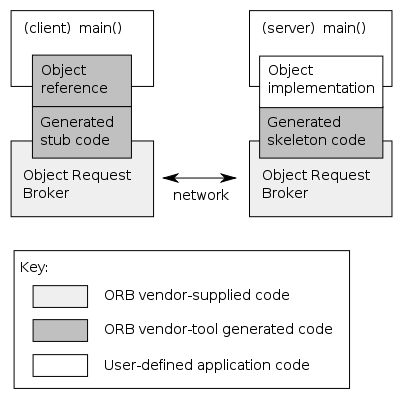
\includegraphics[width=13cm,height=7cm]{401px-Orb.png}
	   \caption{Model de Client-servidor que necesitem}
	   \label{fig:401px-Orb.png}
	   \end{figure} 

	   Tecnologíes per a executar RPCs (Remote procedure call) n'hi ha moltes
	   diferents. Les tecnologies que ens obliguen a utilitzar el mateix llenguatge de
programació han quedat descartades de bon principi, ja que un dels objectius
principals és precisament obrir el programa a futures aplicacions que puguem
crear.  És per això que RMI, que ens lliga a java no pot ser utilitzada.  



\subsection{Algoritme Genètic} % (fold)
	\label{sub:Algoritme Genetic}
% subsection Algoritme Genetic (end)

\subsection{Implementació} % (fold)
	\label{sub:Implementacio}

\begin{itemize}
	\item Els arxius de configuració de eodev es creen amb Template Toolkit
	\item La comunicació amb la bbdd es fa amb DBIX\dots Class
	\item la implementacio de SOAP, s'utilitza SOAP\dots Lite i WSDL\dots SOAP.
		Soap vs REST
	\item MysQl vs TC vs MongoDB
\end{itemize}


% subsection Implementació (end)

% section Procediment informàtic (end)
\section{Resultats} % (fold)
	\label{sec:Resultats}
	\subsection{treball futur} % (fold)
	\label{sub:treball futur}
	implementar tècniques de algorisme genètic  interactius
	
	% subsection treball futur (end)
% section Resultats (end)
\end{document}
